% Options for packages loaded elsewhere
\PassOptionsToPackage{unicode}{hyperref}
\PassOptionsToPackage{hyphens}{url}
\PassOptionsToPackage{dvipsnames,svgnames,x11names}{xcolor}
%
\documentclass[
]{article}

\usepackage{amsmath,amssymb}
\usepackage{iftex}
\ifPDFTeX
  \usepackage[T1]{fontenc}
  \usepackage[utf8]{inputenc}
  \usepackage{textcomp} % provide euro and other symbols
\else % if luatex or xetex
  \usepackage{unicode-math}
  \defaultfontfeatures{Scale=MatchLowercase}
  \defaultfontfeatures[\rmfamily]{Ligatures=TeX,Scale=1}
\fi
\usepackage[]{times}
\ifPDFTeX\else  
    % xetex/luatex font selection
\fi
% Use upquote if available, for straight quotes in verbatim environments
\IfFileExists{upquote.sty}{\usepackage{upquote}}{}
\IfFileExists{microtype.sty}{% use microtype if available
  \usepackage[]{microtype}
  \UseMicrotypeSet[protrusion]{basicmath} % disable protrusion for tt fonts
}{}
\makeatletter
\@ifundefined{KOMAClassName}{% if non-KOMA class
  \IfFileExists{parskip.sty}{%
    \usepackage{parskip}
  }{% else
    \setlength{\parindent}{0pt}
    \setlength{\parskip}{6pt plus 2pt minus 1pt}}
}{% if KOMA class
  \KOMAoptions{parskip=half}}
\makeatother
\usepackage{xcolor}
\setlength{\emergencystretch}{3em} % prevent overfull lines
\setcounter{secnumdepth}{2}
% Make \paragraph and \subparagraph free-standing
\makeatletter
\ifx\paragraph\undefined\else
  \let\oldparagraph\paragraph
  \renewcommand{\paragraph}{
    \@ifstar
      \xxxParagraphStar
      \xxxParagraphNoStar
  }
  \newcommand{\xxxParagraphStar}[1]{\oldparagraph*{#1}\mbox{}}
  \newcommand{\xxxParagraphNoStar}[1]{\oldparagraph{#1}\mbox{}}
\fi
\ifx\subparagraph\undefined\else
  \let\oldsubparagraph\subparagraph
  \renewcommand{\subparagraph}{
    \@ifstar
      \xxxSubParagraphStar
      \xxxSubParagraphNoStar
  }
  \newcommand{\xxxSubParagraphStar}[1]{\oldsubparagraph*{#1}\mbox{}}
  \newcommand{\xxxSubParagraphNoStar}[1]{\oldsubparagraph{#1}\mbox{}}
\fi
\makeatother


\providecommand{\tightlist}{%
  \setlength{\itemsep}{0pt}\setlength{\parskip}{0pt}}\usepackage{longtable,booktabs,array}
\usepackage{calc} % for calculating minipage widths
% Correct order of tables after \paragraph or \subparagraph
\usepackage{etoolbox}
\makeatletter
\patchcmd\longtable{\par}{\if@noskipsec\mbox{}\fi\par}{}{}
\makeatother
% Allow footnotes in longtable head/foot
\IfFileExists{footnotehyper.sty}{\usepackage{footnotehyper}}{\usepackage{footnote}}
\makesavenoteenv{longtable}
\usepackage{graphicx}
\makeatletter
\def\maxwidth{\ifdim\Gin@nat@width>\linewidth\linewidth\else\Gin@nat@width\fi}
\def\maxheight{\ifdim\Gin@nat@height>\textheight\textheight\else\Gin@nat@height\fi}
\makeatother
% Scale images if necessary, so that they will not overflow the page
% margins by default, and it is still possible to overwrite the defaults
% using explicit options in \includegraphics[width, height, ...]{}
\setkeys{Gin}{width=\maxwidth,height=\maxheight,keepaspectratio}
% Set default figure placement to htbp
\makeatletter
\def\fps@figure{htbp}
\makeatother
% definitions for citeproc citations
\NewDocumentCommand\citeproctext{}{}
\NewDocumentCommand\citeproc{mm}{%
  \begingroup\def\citeproctext{#2}\cite{#1}\endgroup}
\makeatletter
 % allow citations to break across lines
 \let\@cite@ofmt\@firstofone
 % avoid brackets around text for \cite:
 \def\@biblabel#1{}
 \def\@cite#1#2{{#1\if@tempswa , #2\fi}}
\makeatother
\newlength{\cslhangindent}
\setlength{\cslhangindent}{1.5em}
\newlength{\csllabelwidth}
\setlength{\csllabelwidth}{3em}
\newenvironment{CSLReferences}[2] % #1 hanging-indent, #2 entry-spacing
 {\begin{list}{}{%
  \setlength{\itemindent}{0pt}
  \setlength{\leftmargin}{0pt}
  \setlength{\parsep}{0pt}
  % turn on hanging indent if param 1 is 1
  \ifodd #1
   \setlength{\leftmargin}{\cslhangindent}
   \setlength{\itemindent}{-1\cslhangindent}
  \fi
  % set entry spacing
  \setlength{\itemsep}{#2\baselineskip}}}
 {\end{list}}
\usepackage{calc}
\newcommand{\CSLBlock}[1]{\hfill\break\parbox[t]{\linewidth}{\strut\ignorespaces#1\strut}}
\newcommand{\CSLLeftMargin}[1]{\parbox[t]{\csllabelwidth}{\strut#1\strut}}
\newcommand{\CSLRightInline}[1]{\parbox[t]{\linewidth - \csllabelwidth}{\strut#1\strut}}
\newcommand{\CSLIndent}[1]{\hspace{\cslhangindent}#1}

% Place figures and tables exactly where they were called
\usepackage{float}
\floatplacement{figure}{H}
\floatplacement{table}{H}

% Recommended by the modelsummary package
\usepackage{booktabs}
\usepackage{siunitx}
\newcolumntype{d}{S[input-symbols = ()]}

% Add affiliations (title.tex needs to be called under template-partials)
\usepackage[noblocks]{authblk}
\renewcommand*{\Authsep}{, }
\renewcommand*{\Authand}{, }
\renewcommand*{\Authands}{, }
\renewcommand\Affilfont{\small}

% Add line numbers
\usepackage{lineno}
\linenumbers
\usepackage{fontspec}
\usepackage{multirow}
\usepackage{multicol}
\usepackage{colortbl}
\usepackage{hhline}
\newlength\Oldarrayrulewidth
\newlength\Oldtabcolsep
\usepackage{longtable}
\usepackage{array}
\usepackage{hyperref}
\usepackage{float}
\usepackage{wrapfig}
\makeatletter
\@ifpackageloaded{caption}{}{\usepackage{caption}}
\AtBeginDocument{%
\ifdefined\contentsname
  \renewcommand*\contentsname{Table of contents}
\else
  \newcommand\contentsname{Table of contents}
\fi
\ifdefined\listfigurename
  \renewcommand*\listfigurename{List of Figures}
\else
  \newcommand\listfigurename{List of Figures}
\fi
\ifdefined\listtablename
  \renewcommand*\listtablename{List of Tables}
\else
  \newcommand\listtablename{List of Tables}
\fi
\ifdefined\figurename
  \renewcommand*\figurename{Figure}
\else
  \newcommand\figurename{Figure}
\fi
\ifdefined\tablename
  \renewcommand*\tablename{Table}
\else
  \newcommand\tablename{Table}
\fi
}
\@ifpackageloaded{float}{}{\usepackage{float}}
\floatstyle{ruled}
\@ifundefined{c@chapter}{\newfloat{codelisting}{h}{lop}}{\newfloat{codelisting}{h}{lop}[chapter]}
\floatname{codelisting}{Listing}
\newcommand*\listoflistings{\listof{codelisting}{List of Listings}}
\makeatother
\makeatletter
\makeatother
\makeatletter
\@ifpackageloaded{caption}{}{\usepackage{caption}}
\@ifpackageloaded{subcaption}{}{\usepackage{subcaption}}
\makeatother

\ifLuaTeX
  \usepackage{selnolig}  % disable illegal ligatures
\fi
\usepackage{bookmark}

\IfFileExists{xurl.sty}{\usepackage{xurl}}{} % add URL line breaks if available
\urlstyle{same} % disable monospaced font for URLs
\hypersetup{
  pdftitle={Evaluating the Profitability of Corn Seeding Decisions: ~Insights from On-Farm Precision Experiments Data},
  pdfauthor={Jaeseok Hwang; Taro Mieno; David S Bullock},
  pdfkeywords={EOSR, OFPE, Yield Seed Response},
  colorlinks=true,
  linkcolor={blue},
  filecolor={Maroon},
  citecolor={red},
  urlcolor={Blue},
  pdfcreator={LaTeX via pandoc}}


\title{Evaluating the Profitability of Corn Seeding Decisions: ~Insights
from On-Farm Precision Experiments Data}


  \author{Jaeseok Hwang}
            \affil{%
                  University of Illinois at Urbana Champaign
              }
        \author{Taro Mieno}
            \affil{%
                  University of Nebraska-Lincoln
              }
        \author{David S Bullock}
            \affil{%
                  University of Illinois at Urbana Champaign
              }
      
\date{2024-10-09}
\begin{document}
\maketitle
\begin{abstract}
Efficient input use is a critical challenge in modern agriculture,
particularly as farmers seek to balance productivity with cost
management. In many of U.S. corn fields, farmers often apply seeding
rates based on their own historical practices rather than data-driven
economic optimization, leading to potential inaccurate input
application. This research addresses the question of how profitable
current corn seeding decisions are and whether farmers could increase
profitability by estimating yield seed(S) response and Economically
Otimal Seeding Rates (EOSR) with the On-Farm Precision Experiment
(OFPE). Using data from 97 OFPE trials conducted between 2016 and 2023,
this study contrasts farmers' status quo seeding rates (SQSR) with EOSR
estimates derived from Generalized Additive Model (GAM) regression.
Results indicate that, on average, farmers overapply by 3.8K seeds per
acre, leading to an average loss of \$24.7 per acre in 40 percent of the
trials. The analysis provides evidence for high-rate seeding practices
to enhance profitability, with potential implications for agricultural
policy or extension.
\end{abstract}


\newpage

\section{Introduction}\label{introduction}

From the early 1970s, for about 50 years, maize yield in U.S. has been
gradually increasing and it almost doubled, from 91.3 in 1973 to 177.3
bushels per acre in 2023 ((\citeproc{ref-usdanass}{1})). This
considerable growth in yield attributes to innovations in genotype,
environment and management but still it is not clear how much each
factors contribute to yield increase since their interactions in yield
responses are very complicated((\citeproc{ref-morris2018strengths}{2})).
The main drivers of the yield increase are, however, the improvement of
genetically engineered seed and hybrid seed. These innovations in seed
technology enables higher density of seed population endure stress of
competition within a given area of planting and it drastically increases
the probability of germination
((\citeproc{ref-fernandez2014genetically}{3})). Therefore, raising the
seeding rate with the improved seed varieties promote the per acre corn
yield to the current level.

The increase in yield enhances the net revenue of farmer, with the
relatively cheap cost of seed, while the seeding rate has increased
during the late 20th century for 30years, from 1970s to 1990s. However,
from the 2000s, there has been a fluctuation in seed cost and the
portion of the seed cost in the total operation cost increased a lot
((\citeproc{ref-saavoss2021trends}{4})). As a result, the portion of
total seed cost and fertilizer cost in the operation cost became much
closer, and the benefit of the estimated Economically Optimum Seeding
Rate (EOSR) has been increased in terms of saving operation cost and
enhancing total revenue of corn production.

\begin{figure}[H]

{\centering 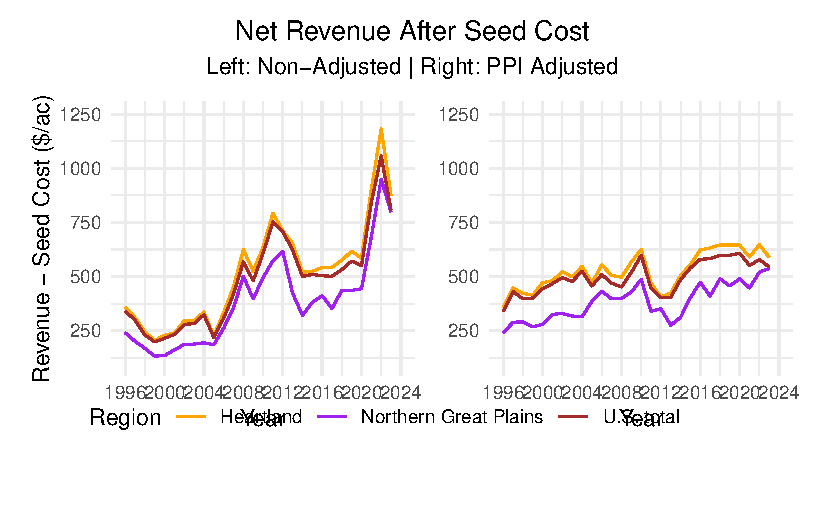
\includegraphics[width=0.8\textwidth,height=0.8\textheight]{corn_seed_response_writing_files/figure-pdf/fig1-rev-seed-comb-1.pdf}

}

\caption{Net revenue after seed cost figure 1996 to 2023}

\end{figure}%

However, despite of this increasing burden of seed cost, farmers do not
frequently adjust their seeding rates with respect to their very recent
variation in market price and weather
condition((\citeproc{ref-usdanass}{1})). Also,
(\citeproc{ref-usdanass}{1}) data shows the evidence that the farmers do
not really adjust their seeding rate during the time that the corn price
decreases, while the seed cost increases and per acre revenue decreases.
Figure (\citeproc{ref-fig1-rev-seed-comb}{\textbf{fig1-rev-seed-comb?}})
shows the trend of the yearly changes of net revenue after seed cost
over the recent 30 years. The left plot shows the continuous increase in
net revenue over 30 years, however, when we adjust it by Producer Price
Index(PPI) of corn in agricultural commodity sector, the net revenue
stops increasing from 2016 and there are high fluctuation and decreasing
trend of net revenue very recently.

In various recent resources, the estimated EOSR on the midwest Corn-belt
(Heartland) are ranged from 32k to 36k
((\citeproc{ref-illinois2023seed}{5}),(\citeproc{ref-licht2017corn}{6}),(\citeproc{ref-lindsey2018modeling}{7}),(\citeproc{ref-nielsen2019yield}{8}),(\citeproc{ref-lacasa2020bayesian}{9})).
For instance, (\citeproc{ref-assefa2018analysis}{10}) estimated EOSR
with the 14 years of on-farm experimental results from 22 different
states, and it recommend 34K as a EOSR in the moderate weather condition
in the Midwest corn-belt. However, the impact of recently increased
draught and extreme weather decreases the probability of high attainable
yield in many of the Midwest fields and it doubt the profitability of
the aforementioned high rates, 34K, seeding
((\citeproc{ref-kukal2018climate}{11}),(\citeproc{ref-rigden2020combined}{12})).

This research, hence, investigate how much the farmer's choice of corn
seeding rate are profitable with the recent empirical On-Farm Precision
Experiment(OFPE) data which are collected from 2016 to 2023 over 8
different states in U.S. To evaluate the profit of farmer's status quo
seeding rate (SQSR), yield seed(S) response function for each experiment
fields are calculated by the Generalized Additive Model(GAM) regression.
Then, the estimated profits of SQSRs and estimated EOSRs are evaluated
by the type of yield S response and seeding rate differences in SQSR and
EOSR.

The result find out the evidence that the farmers are likely to plant
about 3.8K more seed than estimated EOSR, and at the 40 out of 100
participated trials, farmers loss about \$24.7 per acre potential profit
due to excessive high seeding decision behavior.

\section{Method}\label{method}

\subsection{Datasets}\label{datasets}

This research mainly evaluates the estimated profit of farmer's SQSR and
EOSR by projecting it on the given climate conditions. To estimate the
profit at the SQSR and EOSR accurately, it is requisite to estimate
field specific yield S response function. Thus, to estimate yield S
response of the experimental fields, OFPE data were collected and
processed by the following steps.

First, 163 OFPE data was adopted from the database that is collected by
the Data Intensive Farm Management (DIFM) project
(\citeproc{ref-bullock2019data}{13}). The 169 dataset was gathered from
the 42 farms which are located on 8 differents state of Midwest
Corn-belt. DIFM project consults OFPE by designing S x N trial input
combination to be applied and planted into trial polygon, and it
prevents seed and nitrogen having spatial correlation. Also, these two
controlled inputs are spatially independent with soil and field specific
characteristics (\citeproc{ref-lix2021design}{14}).

\begin{figure}[H]

{\centering 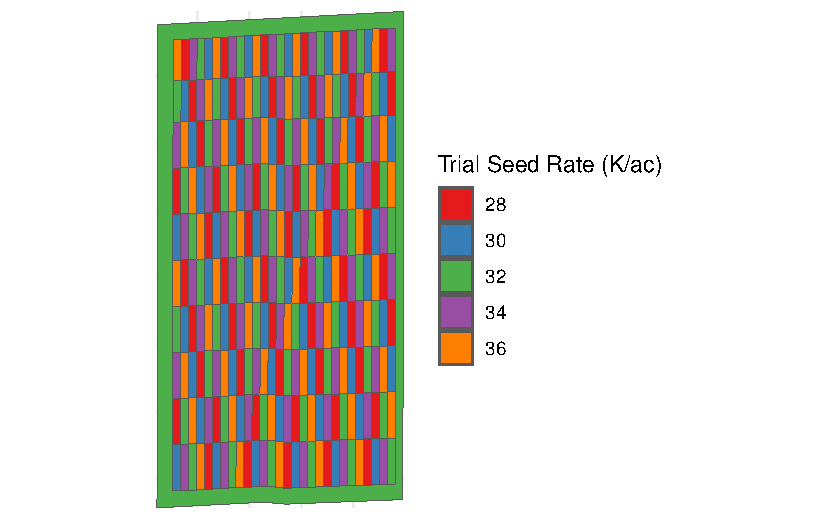
\includegraphics[width=17.1875in,height=\textheight]{corn_seed_response_writing_files/figure-pdf/fig2-td-sample-1.pdf}

}

\caption{On Farm Trial Design Sample}

\end{figure}%

Figure (\citeproc{ref-fig2-td-sample}{\textbf{fig2-td-sample?}}) shows
the example of the design, and the range of trial inputs are determined
by assigning farmer's SQSR into the middle of the trial inputs range.
Following this trial-design, farmers apply the assigned rates and
harvest the crop by using GPS-linked vehicle, and it records the S , N
and yield data in real-time. The experimental data, yield, S and N are
cleaned and processed by the protocol in
(\citeproc{ref-edge2024processing}{15}). The protocol creates yield
polygon by eliminating the highly deviated or the misaligned yield
points. The size of the yield polygon is determined by the size of the
trial polygon, swath-width and distance of the harvester, applicator and
planter. Input polygons for S and N are created by removing outliers and
the data points which are located in the transition zone where the
vehicle changes the trial rate. After this individual cleaning process,
it calculates the median value of input polygons into yield polygons to
combine yield and input polygon. At this process, the yield polygon
where the combined input polygon have high deviation are removed to
prevent input straddling problem. Through this cleaning protocol, 66 out
of 163 OFPE data are excluded in the dataset since they have too small
observations due to straddling problem or errors in the field-collected
raw level data.

\global\setlength{\Oldarrayrulewidth}{\arrayrulewidth}

\global\setlength{\Oldtabcolsep}{\tabcolsep}

\setlength{\tabcolsep}{2pt}

\renewcommand*{\arraystretch}{1.5}



\providecommand{\ascline}[3]{\noalign{\global\arrayrulewidth #1}\arrayrulecolor[HTML]{#2}\cline{#3}}

\begin{longtable*}[c]{ccccccccc}



\ascline{1.5pt}{666666}{1-9}

\multicolumn{1}{>{}c}{\textcolor[HTML]{000000}{\fontsize{11}{11}\selectfont{Year}}} & \multicolumn{1}{>{}c}{\textcolor[HTML]{000000}{\fontsize{11}{11}\selectfont{Field}}\textcolor[HTML]{000000}{\fontsize{11}{11}\selectfont{\linebreak }}\textcolor[HTML]{000000}{\fontsize{11}{11}\selectfont{Count}}} & \multicolumn{1}{>{}c}{\textcolor[HTML]{000000}{\fontsize{11}{11}\selectfont{Mean}}\textcolor[HTML]{000000}{\fontsize{11}{11}\selectfont{\linebreak }}\textcolor[HTML]{000000}{\fontsize{11}{11}\selectfont{Yield}}\textcolor[HTML]{000000}{\fontsize{11}{11}\selectfont{\linebreak }}\textcolor[HTML]{000000}{\fontsize{11}{11}\selectfont{(bu/ac)}}} & \multicolumn{1}{>{}c}{\textcolor[HTML]{000000}{\fontsize{11}{11}\selectfont{SQSR}}} & \multicolumn{1}{>{}c}{\textcolor[HTML]{000000}{\fontsize{11}{11}\selectfont{USDA}}\textcolor[HTML]{000000}{\fontsize{11}{11}\selectfont{\linebreak }}\textcolor[HTML]{000000}{\fontsize{11}{11}\selectfont{SR}}} & \multicolumn{1}{>{}c}{\textcolor[HTML]{000000}{\fontsize{11}{11}\selectfont{Precipitation}}\textcolor[HTML]{000000}{\fontsize{11}{11}\selectfont{\linebreak }}\textcolor[HTML]{000000}{\fontsize{11}{11}\selectfont{(In-Season)}}} & \multicolumn{1}{>{}c}{\textcolor[HTML]{000000}{\fontsize{11}{11}\selectfont{GDD}}\textcolor[HTML]{000000}{\fontsize{11}{11}\selectfont{\linebreak }}\textcolor[HTML]{000000}{\fontsize{11}{11}\selectfont{(In-Season)}}} & \multicolumn{1}{>{}c}{\textcolor[HTML]{000000}{\fontsize{11}{11}\selectfont{Precipitation}}\textcolor[HTML]{000000}{\fontsize{11}{11}\selectfont{\linebreak }}\textcolor[HTML]{000000}{\fontsize{11}{11}\selectfont{(30Year)}}} & \multicolumn{1}{>{}c}{\textcolor[HTML]{000000}{\fontsize{11}{11}\selectfont{GDD}}\textcolor[HTML]{000000}{\fontsize{11}{11}\selectfont{\linebreak }}\textcolor[HTML]{000000}{\fontsize{11}{11}\selectfont{(30Year)}}} \\

\ascline{1.5pt}{666666}{1-9}\endfirsthead 

\ascline{1.5pt}{666666}{1-9}

\multicolumn{1}{>{}c}{\textcolor[HTML]{000000}{\fontsize{11}{11}\selectfont{Year}}} & \multicolumn{1}{>{}c}{\textcolor[HTML]{000000}{\fontsize{11}{11}\selectfont{Field}}\textcolor[HTML]{000000}{\fontsize{11}{11}\selectfont{\linebreak }}\textcolor[HTML]{000000}{\fontsize{11}{11}\selectfont{Count}}} & \multicolumn{1}{>{}c}{\textcolor[HTML]{000000}{\fontsize{11}{11}\selectfont{Mean}}\textcolor[HTML]{000000}{\fontsize{11}{11}\selectfont{\linebreak }}\textcolor[HTML]{000000}{\fontsize{11}{11}\selectfont{Yield}}\textcolor[HTML]{000000}{\fontsize{11}{11}\selectfont{\linebreak }}\textcolor[HTML]{000000}{\fontsize{11}{11}\selectfont{(bu/ac)}}} & \multicolumn{1}{>{}c}{\textcolor[HTML]{000000}{\fontsize{11}{11}\selectfont{SQSR}}} & \multicolumn{1}{>{}c}{\textcolor[HTML]{000000}{\fontsize{11}{11}\selectfont{USDA}}\textcolor[HTML]{000000}{\fontsize{11}{11}\selectfont{\linebreak }}\textcolor[HTML]{000000}{\fontsize{11}{11}\selectfont{SR}}} & \multicolumn{1}{>{}c}{\textcolor[HTML]{000000}{\fontsize{11}{11}\selectfont{Precipitation}}\textcolor[HTML]{000000}{\fontsize{11}{11}\selectfont{\linebreak }}\textcolor[HTML]{000000}{\fontsize{11}{11}\selectfont{(In-Season)}}} & \multicolumn{1}{>{}c}{\textcolor[HTML]{000000}{\fontsize{11}{11}\selectfont{GDD}}\textcolor[HTML]{000000}{\fontsize{11}{11}\selectfont{\linebreak }}\textcolor[HTML]{000000}{\fontsize{11}{11}\selectfont{(In-Season)}}} & \multicolumn{1}{>{}c}{\textcolor[HTML]{000000}{\fontsize{11}{11}\selectfont{Precipitation}}\textcolor[HTML]{000000}{\fontsize{11}{11}\selectfont{\linebreak }}\textcolor[HTML]{000000}{\fontsize{11}{11}\selectfont{(30Year)}}} & \multicolumn{1}{>{}c}{\textcolor[HTML]{000000}{\fontsize{11}{11}\selectfont{GDD}}\textcolor[HTML]{000000}{\fontsize{11}{11}\selectfont{\linebreak }}\textcolor[HTML]{000000}{\fontsize{11}{11}\selectfont{(30Year)}}} \\

\ascline{1.5pt}{666666}{1-9}\endhead



\multicolumn{1}{>{}c}{\textcolor[HTML]{000000}{\fontsize{11}{11}\selectfont{2,016}}} & \multicolumn{1}{>{}c}{\textcolor[HTML]{000000}{\fontsize{11}{11}\selectfont{4}}} & \multicolumn{1}{>{}c}{\textcolor[HTML]{000000}{\fontsize{11}{11}\selectfont{178.9}}\textcolor[HTML]{000000}{\fontsize{11}{11}\selectfont{\linebreak }}\textcolor[HTML]{000000}{\fontsize{11}{11}\selectfont{(59.7)}}} & \multicolumn{1}{>{}c}{\textcolor[HTML]{000000}{\fontsize{11}{11}\selectfont{35.5}}\textcolor[HTML]{000000}{\fontsize{11}{11}\selectfont{\linebreak }}\textcolor[HTML]{000000}{\fontsize{11}{11}\selectfont{(0.6)}}} & \multicolumn{1}{>{}c}{\textcolor[HTML]{000000}{\fontsize{11}{11}\selectfont{31.1}}\textcolor[HTML]{000000}{\fontsize{11}{11}\selectfont{\linebreak }}\textcolor[HTML]{000000}{\fontsize{11}{11}\selectfont{(0.0)}}} & \multicolumn{1}{>{}c}{\textcolor[HTML]{000000}{\fontsize{11}{11}\selectfont{787.7}}\textcolor[HTML]{000000}{\fontsize{11}{11}\selectfont{\linebreak }}\textcolor[HTML]{000000}{\fontsize{11}{11}\selectfont{(38.0)}}} & \multicolumn{1}{>{}c}{\textcolor[HTML]{000000}{\fontsize{11}{11}\selectfont{2000.5}}\textcolor[HTML]{000000}{\fontsize{11}{11}\selectfont{\linebreak }}\textcolor[HTML]{000000}{\fontsize{11}{11}\selectfont{(95.3)}}} & \multicolumn{1}{>{}c}{\textcolor[HTML]{000000}{\fontsize{11}{11}\selectfont{646.3}}\textcolor[HTML]{000000}{\fontsize{11}{11}\selectfont{\linebreak }}\textcolor[HTML]{000000}{\fontsize{11}{11}\selectfont{(26.8)}}} & \multicolumn{1}{>{}c}{\textcolor[HTML]{000000}{\fontsize{11}{11}\selectfont{1871.0}}\textcolor[HTML]{000000}{\fontsize{11}{11}\selectfont{\linebreak }}\textcolor[HTML]{000000}{\fontsize{11}{11}\selectfont{(81.4)}}} \\





\multicolumn{1}{>{}c}{\textcolor[HTML]{000000}{\fontsize{11}{11}\selectfont{2,017}}} & \multicolumn{1}{>{}c}{\textcolor[HTML]{000000}{\fontsize{11}{11}\selectfont{6}}} & \multicolumn{1}{>{}c}{\textcolor[HTML]{000000}{\fontsize{11}{11}\selectfont{227.0}}\textcolor[HTML]{000000}{\fontsize{11}{11}\selectfont{\linebreak }}\textcolor[HTML]{000000}{\fontsize{11}{11}\selectfont{(29.3)}}} & \multicolumn{1}{>{}c}{\textcolor[HTML]{000000}{\fontsize{11}{11}\selectfont{34.5}}\textcolor[HTML]{000000}{\fontsize{11}{11}\selectfont{\linebreak }}\textcolor[HTML]{000000}{\fontsize{11}{11}\selectfont{(1.4)}}} & \multicolumn{1}{>{}c}{\textcolor[HTML]{000000}{\fontsize{11}{11}\selectfont{30.6}}\textcolor[HTML]{000000}{\fontsize{11}{11}\selectfont{\linebreak }}\textcolor[HTML]{000000}{\fontsize{11}{11}\selectfont{(0.8)}}} & \multicolumn{1}{>{}c}{\textcolor[HTML]{000000}{\fontsize{11}{11}\selectfont{611.9}}\textcolor[HTML]{000000}{\fontsize{11}{11}\selectfont{\linebreak }}\textcolor[HTML]{000000}{\fontsize{11}{11}\selectfont{(65.9)}}} & \multicolumn{1}{>{}c}{\textcolor[HTML]{000000}{\fontsize{11}{11}\selectfont{1825.6}}\textcolor[HTML]{000000}{\fontsize{11}{11}\selectfont{\linebreak }}\textcolor[HTML]{000000}{\fontsize{11}{11}\selectfont{(159.4)}}} & \multicolumn{1}{>{}c}{\textcolor[HTML]{000000}{\fontsize{11}{11}\selectfont{631.4}}\textcolor[HTML]{000000}{\fontsize{11}{11}\selectfont{\linebreak }}\textcolor[HTML]{000000}{\fontsize{11}{11}\selectfont{(26.0)}}} & \multicolumn{1}{>{}c}{\textcolor[HTML]{000000}{\fontsize{11}{11}\selectfont{1801.7}}\textcolor[HTML]{000000}{\fontsize{11}{11}\selectfont{\linebreak }}\textcolor[HTML]{000000}{\fontsize{11}{11}\selectfont{(152.0)}}} \\





\multicolumn{1}{>{}c}{\textcolor[HTML]{000000}{\fontsize{11}{11}\selectfont{2,018}}} & \multicolumn{1}{>{}c}{\textcolor[HTML]{000000}{\fontsize{11}{11}\selectfont{12}}} & \multicolumn{1}{>{}c}{\textcolor[HTML]{000000}{\fontsize{11}{11}\selectfont{231.8}}\textcolor[HTML]{000000}{\fontsize{11}{11}\selectfont{\linebreak }}\textcolor[HTML]{000000}{\fontsize{11}{11}\selectfont{(23.6)}}} & \multicolumn{1}{>{}c}{\textcolor[HTML]{000000}{\fontsize{11}{11}\selectfont{35.0}}\textcolor[HTML]{000000}{\fontsize{11}{11}\selectfont{\linebreak }}\textcolor[HTML]{000000}{\fontsize{11}{11}\selectfont{(1.0)}}} & \multicolumn{1}{>{}c}{\textcolor[HTML]{000000}{\fontsize{11}{11}\selectfont{31.5}}\textcolor[HTML]{000000}{\fontsize{11}{11}\selectfont{\linebreak }}\textcolor[HTML]{000000}{\fontsize{11}{11}\selectfont{(0.8)}}} & \multicolumn{1}{>{}c}{\textcolor[HTML]{000000}{\fontsize{11}{11}\selectfont{656.5}}\textcolor[HTML]{000000}{\fontsize{11}{11}\selectfont{\linebreak }}\textcolor[HTML]{000000}{\fontsize{11}{11}\selectfont{(100.2)}}} & \multicolumn{1}{>{}c}{\textcolor[HTML]{000000}{\fontsize{11}{11}\selectfont{1919.5}}\textcolor[HTML]{000000}{\fontsize{11}{11}\selectfont{\linebreak }}\textcolor[HTML]{000000}{\fontsize{11}{11}\selectfont{(169.9)}}} & \multicolumn{1}{>{}c}{\textcolor[HTML]{000000}{\fontsize{11}{11}\selectfont{630.4}}\textcolor[HTML]{000000}{\fontsize{11}{11}\selectfont{\linebreak }}\textcolor[HTML]{000000}{\fontsize{11}{11}\selectfont{(29.6)}}} & \multicolumn{1}{>{}c}{\textcolor[HTML]{000000}{\fontsize{11}{11}\selectfont{1710.9}}\textcolor[HTML]{000000}{\fontsize{11}{11}\selectfont{\linebreak }}\textcolor[HTML]{000000}{\fontsize{11}{11}\selectfont{(179.7)}}} \\





\multicolumn{1}{>{}c}{\textcolor[HTML]{000000}{\fontsize{11}{11}\selectfont{2,019}}} & \multicolumn{1}{>{}c}{\textcolor[HTML]{000000}{\fontsize{11}{11}\selectfont{8}}} & \multicolumn{1}{>{}c}{\textcolor[HTML]{000000}{\fontsize{11}{11}\selectfont{186.4}}\textcolor[HTML]{000000}{\fontsize{11}{11}\selectfont{\linebreak }}\textcolor[HTML]{000000}{\fontsize{11}{11}\selectfont{(27.2)}}} & \multicolumn{1}{>{}c}{\textcolor[HTML]{000000}{\fontsize{11}{11}\selectfont{33.9}}\textcolor[HTML]{000000}{\fontsize{11}{11}\selectfont{\linebreak }}\textcolor[HTML]{000000}{\fontsize{11}{11}\selectfont{(2.1)}}} & \multicolumn{1}{>{}c}{\textcolor[HTML]{000000}{\fontsize{11}{11}\selectfont{30.8}}\textcolor[HTML]{000000}{\fontsize{11}{11}\selectfont{\linebreak }}\textcolor[HTML]{000000}{\fontsize{11}{11}\selectfont{(0.3)}}} & \multicolumn{1}{>{}c}{\textcolor[HTML]{000000}{\fontsize{11}{11}\selectfont{776.6}}\textcolor[HTML]{000000}{\fontsize{11}{11}\selectfont{\linebreak }}\textcolor[HTML]{000000}{\fontsize{11}{11}\selectfont{(117.7)}}} & \multicolumn{1}{>{}c}{\textcolor[HTML]{000000}{\fontsize{11}{11}\selectfont{1791.3}}\textcolor[HTML]{000000}{\fontsize{11}{11}\selectfont{\linebreak }}\textcolor[HTML]{000000}{\fontsize{11}{11}\selectfont{(265.3)}}} & \multicolumn{1}{>{}c}{\textcolor[HTML]{000000}{\fontsize{11}{11}\selectfont{651.0}}\textcolor[HTML]{000000}{\fontsize{11}{11}\selectfont{\linebreak }}\textcolor[HTML]{000000}{\fontsize{11}{11}\selectfont{(27.1)}}} & \multicolumn{1}{>{}c}{\textcolor[HTML]{000000}{\fontsize{11}{11}\selectfont{1715.2}}\textcolor[HTML]{000000}{\fontsize{11}{11}\selectfont{\linebreak }}\textcolor[HTML]{000000}{\fontsize{11}{11}\selectfont{(240.9)}}} \\





\multicolumn{1}{>{}c}{\textcolor[HTML]{000000}{\fontsize{11}{11}\selectfont{2,020}}} & \multicolumn{1}{>{}c}{\textcolor[HTML]{000000}{\fontsize{11}{11}\selectfont{10}}} & \multicolumn{1}{>{}c}{\textcolor[HTML]{000000}{\fontsize{11}{11}\selectfont{192.5}}\textcolor[HTML]{000000}{\fontsize{11}{11}\selectfont{\linebreak }}\textcolor[HTML]{000000}{\fontsize{11}{11}\selectfont{(42.3)}}} & \multicolumn{1}{>{}c}{\textcolor[HTML]{000000}{\fontsize{11}{11}\selectfont{33.4}}\textcolor[HTML]{000000}{\fontsize{11}{11}\selectfont{\linebreak }}\textcolor[HTML]{000000}{\fontsize{11}{11}\selectfont{(3.5)}}} & \multicolumn{1}{>{}c}{\textcolor[HTML]{000000}{\fontsize{11}{11}\selectfont{30.3}}\textcolor[HTML]{000000}{\fontsize{11}{11}\selectfont{\linebreak }}\textcolor[HTML]{000000}{\fontsize{11}{11}\selectfont{(0.2)}}} & \multicolumn{1}{>{}c}{\textcolor[HTML]{000000}{\fontsize{11}{11}\selectfont{598.4}}\textcolor[HTML]{000000}{\fontsize{11}{11}\selectfont{\linebreak }}\textcolor[HTML]{000000}{\fontsize{11}{11}\selectfont{(145.8)}}} & \multicolumn{1}{>{}c}{\textcolor[HTML]{000000}{\fontsize{11}{11}\selectfont{1633.7}}\textcolor[HTML]{000000}{\fontsize{11}{11}\selectfont{\linebreak }}\textcolor[HTML]{000000}{\fontsize{11}{11}\selectfont{(154.4)}}} & \multicolumn{1}{>{}c}{\textcolor[HTML]{000000}{\fontsize{11}{11}\selectfont{626.9}}\textcolor[HTML]{000000}{\fontsize{11}{11}\selectfont{\linebreak }}\textcolor[HTML]{000000}{\fontsize{11}{11}\selectfont{(97.2)}}} & \multicolumn{1}{>{}c}{\textcolor[HTML]{000000}{\fontsize{11}{11}\selectfont{1649.1}}\textcolor[HTML]{000000}{\fontsize{11}{11}\selectfont{\linebreak }}\textcolor[HTML]{000000}{\fontsize{11}{11}\selectfont{(218.9)}}} \\





\multicolumn{1}{>{}c}{\textcolor[HTML]{000000}{\fontsize{11}{11}\selectfont{2,021}}} & \multicolumn{1}{>{}c}{\textcolor[HTML]{000000}{\fontsize{11}{11}\selectfont{14}}} & \multicolumn{1}{>{}c}{\textcolor[HTML]{000000}{\fontsize{11}{11}\selectfont{198.2}}\textcolor[HTML]{000000}{\fontsize{11}{11}\selectfont{\linebreak }}\textcolor[HTML]{000000}{\fontsize{11}{11}\selectfont{(41.7)}}} & \multicolumn{1}{>{}c}{\textcolor[HTML]{000000}{\fontsize{11}{11}\selectfont{33.0}}\textcolor[HTML]{000000}{\fontsize{11}{11}\selectfont{\linebreak }}\textcolor[HTML]{000000}{\fontsize{11}{11}\selectfont{(2.7)}}} & \multicolumn{1}{>{}c}{\textcolor[HTML]{000000}{\fontsize{11}{11}\selectfont{30.4}}\textcolor[HTML]{000000}{\fontsize{11}{11}\selectfont{\linebreak }}\textcolor[HTML]{000000}{\fontsize{11}{11}\selectfont{(2.0)}}} & \multicolumn{1}{>{}c}{\textcolor[HTML]{000000}{\fontsize{11}{11}\selectfont{618.6}}\textcolor[HTML]{000000}{\fontsize{11}{11}\selectfont{\linebreak }}\textcolor[HTML]{000000}{\fontsize{11}{11}\selectfont{(145.6)}}} & \multicolumn{1}{>{}c}{\textcolor[HTML]{000000}{\fontsize{11}{11}\selectfont{1811.0}}\textcolor[HTML]{000000}{\fontsize{11}{11}\selectfont{\linebreak }}\textcolor[HTML]{000000}{\fontsize{11}{11}\selectfont{(117.0)}}} & \multicolumn{1}{>{}c}{\textcolor[HTML]{000000}{\fontsize{11}{11}\selectfont{616.5}}\textcolor[HTML]{000000}{\fontsize{11}{11}\selectfont{\linebreak }}\textcolor[HTML]{000000}{\fontsize{11}{11}\selectfont{(59.0)}}} & \multicolumn{1}{>{}c}{\textcolor[HTML]{000000}{\fontsize{11}{11}\selectfont{1732.3}}\textcolor[HTML]{000000}{\fontsize{11}{11}\selectfont{\linebreak }}\textcolor[HTML]{000000}{\fontsize{11}{11}\selectfont{(179.0)}}} \\





\multicolumn{1}{>{}c}{\textcolor[HTML]{000000}{\fontsize{11}{11}\selectfont{2,022}}} & \multicolumn{1}{>{}c}{\textcolor[HTML]{000000}{\fontsize{11}{11}\selectfont{20}}} & \multicolumn{1}{>{}c}{\textcolor[HTML]{000000}{\fontsize{11}{11}\selectfont{187.5}}\textcolor[HTML]{000000}{\fontsize{11}{11}\selectfont{\linebreak }}\textcolor[HTML]{000000}{\fontsize{11}{11}\selectfont{(60.1)}}} & \multicolumn{1}{>{}c}{\textcolor[HTML]{000000}{\fontsize{11}{11}\selectfont{32.4}}\textcolor[HTML]{000000}{\fontsize{11}{11}\selectfont{\linebreak }}\textcolor[HTML]{000000}{\fontsize{11}{11}\selectfont{(3.3)}}} & \multicolumn{1}{>{}c}{\textcolor[HTML]{000000}{\fontsize{11}{11}\selectfont{29.4}}\textcolor[HTML]{000000}{\fontsize{11}{11}\selectfont{\linebreak }}\textcolor[HTML]{000000}{\fontsize{11}{11}\selectfont{(3.2)}}} & \multicolumn{1}{>{}c}{\textcolor[HTML]{000000}{\fontsize{11}{11}\selectfont{484.4}}\textcolor[HTML]{000000}{\fontsize{11}{11}\selectfont{\linebreak }}\textcolor[HTML]{000000}{\fontsize{11}{11}\selectfont{(109.6)}}} & \multicolumn{1}{>{}c}{\textcolor[HTML]{000000}{\fontsize{11}{11}\selectfont{1644.0}}\textcolor[HTML]{000000}{\fontsize{11}{11}\selectfont{\linebreak }}\textcolor[HTML]{000000}{\fontsize{11}{11}\selectfont{(154.6)}}} & \multicolumn{1}{>{}c}{\textcolor[HTML]{000000}{\fontsize{11}{11}\selectfont{562.9}}\textcolor[HTML]{000000}{\fontsize{11}{11}\selectfont{\linebreak }}\textcolor[HTML]{000000}{\fontsize{11}{11}\selectfont{(94.6)}}} & \multicolumn{1}{>{}c}{\textcolor[HTML]{000000}{\fontsize{11}{11}\selectfont{1570.0}}\textcolor[HTML]{000000}{\fontsize{11}{11}\selectfont{\linebreak }}\textcolor[HTML]{000000}{\fontsize{11}{11}\selectfont{(164.1)}}} \\





\multicolumn{1}{>{}c}{\textcolor[HTML]{000000}{\fontsize{11}{11}\selectfont{2,023}}} & \multicolumn{1}{>{}c}{\textcolor[HTML]{000000}{\fontsize{11}{11}\selectfont{22}}} & \multicolumn{1}{>{}c}{\textcolor[HTML]{000000}{\fontsize{11}{11}\selectfont{201.9}}\textcolor[HTML]{000000}{\fontsize{11}{11}\selectfont{\linebreak }}\textcolor[HTML]{000000}{\fontsize{11}{11}\selectfont{(50.2)}}} & \multicolumn{1}{>{}c}{\textcolor[HTML]{000000}{\fontsize{11}{11}\selectfont{32.4}}\textcolor[HTML]{000000}{\fontsize{11}{11}\selectfont{\linebreak }}\textcolor[HTML]{000000}{\fontsize{11}{11}\selectfont{(3.8)}}} & \multicolumn{1}{>{}c}{\textcolor[HTML]{000000}{\fontsize{11}{11}\selectfont{30.0}}\textcolor[HTML]{000000}{\fontsize{11}{11}\selectfont{\linebreak }}\textcolor[HTML]{000000}{\fontsize{11}{11}\selectfont{(3.0)}}} & \multicolumn{1}{>{}c}{\textcolor[HTML]{000000}{\fontsize{11}{11}\selectfont{478.5}}\textcolor[HTML]{000000}{\fontsize{11}{11}\selectfont{\linebreak }}\textcolor[HTML]{000000}{\fontsize{11}{11}\selectfont{(49.4)}}} & \multicolumn{1}{>{}c}{\textcolor[HTML]{000000}{\fontsize{11}{11}\selectfont{1717.0}}\textcolor[HTML]{000000}{\fontsize{11}{11}\selectfont{\linebreak }}\textcolor[HTML]{000000}{\fontsize{11}{11}\selectfont{(166.3)}}} & \multicolumn{1}{>{}c}{\textcolor[HTML]{000000}{\fontsize{11}{11}\selectfont{603.7}}\textcolor[HTML]{000000}{\fontsize{11}{11}\selectfont{\linebreak }}\textcolor[HTML]{000000}{\fontsize{11}{11}\selectfont{(93.3)}}} & \multicolumn{1}{>{}c}{\textcolor[HTML]{000000}{\fontsize{11}{11}\selectfont{1641.0}}\textcolor[HTML]{000000}{\fontsize{11}{11}\selectfont{\linebreak }}\textcolor[HTML]{000000}{\fontsize{11}{11}\selectfont{(199.7)}}} \\

\ascline{1.5pt}{666666}{1-9}



\end{longtable*}



\arrayrulecolor[HTML]{000000}

\global\setlength{\arrayrulewidth}{\Oldarrayrulewidth}

\global\setlength{\tabcolsep}{\Oldtabcolsep}

\renewcommand*{\arraystretch}{1}

The non-experimental variables of field specific information are added
upon the processed yield and input combined polygon. The public data
resource, Soil survey information(SSURGO) and Digital Eleveation
Model(DEM) are used as a field characteristic information; clay, sand,
silt and water storage for soil, elevation, slope and curvature for
topography. The median value of the soil and topography rasters are
calculated for the overlapped polygon of experimental data by using R
software ((\citeproc{ref-r2021language}{16})). As the experimental and
non-experimental variables are cleared and processed, for each
experimental field, in-season (April 1st to September 30th) weather
information is attached. From the Daily surface weather data,
daymet((\citeproc{ref-thornton2022daymet}{17})), in-season total
precipitation and accumulated growing degree day (GDD) of the trial year
are calculated and added on each of the processed OFPE data. Finally,
annual reported average seeding rate by state (USDASR) are obtained from
(\citeproc{ref-usdanass}{1}) and attached to compare the SQSR and USDASR
with the estimated profit, respectively.

Table (\citeproc{ref-tab1-dat-summary}{\textbf{tab1-dat-summary?}}) is
the summary statistics of the processed OFPE data by the trial year
(from 2016 t0 2023). Each row of the table contains the average,
standard deviation, minimum and max value of the experimental data;
yield(bu/ac), SQSR(K/ac), USDASR(K/ac) and weather information;
precipitation(inch) and accumulated GDD.

\subsection{Models}\label{models}

To calculate the profit of farmer's SQSR and EOSR of the trial field,
first, estimating accurate and field specific yield input response
function is important. A number of recent research warns the defining
unique functional form of yield response to input since the function has
diverse form like linear, linear plateau, quadratic, and quadratic
plateau by the field characteristics and weather of the given field and
year ( !!! Add Citation). Thus, this study adopts Generalized Additive
Model(GAM) to estimate yield S response function. To simplify the
analysis and focus on the S rate management, this study consider S as an
only controllable input. GAM has an advantage when the yield response
function has a various form by field since it arbitrary chooses
functional form without making any assumption on input and output
relation.

Equation Equation~\ref{eq-res_f} describes the equation of the yield S
response function.

\begin{equation}\phantomsection\label{eq-res_f}{
y_i = f_i(S, N, Sl, El, As, Tw, Cl, Sn, St, Wt) + \varepsilon_i
}\end{equation}

In equation Equation~\ref{eq-res_f}, \(i\) is an individual field where
OFPE data was collected abd processed. \(y_i\) is the observed yield of
the processed data, and \(f_i\) represents the yield response function
for field \(i\). The function variables of experimental inputs like S
and N, and various non-experimental field characteristics such as
\(Sl\)(slope),\(El\)(elevation),\(As\)(aspect),\(Tw\)(topographic
wetness index) \(Cl\)(clay), \(Sn\)(sand), \(St\)(silt), \(Ws\)(water
storage).

\begin{equation}\phantomsection\label{eq-gam}{
 \hat{f}^{GAM}_{i} \equiv \beta_0+f_{i1}\left(S\right)+f_{i2}\left(N\right)+f_{i3}\left(Sl\right)+f_{i4 }\left(El\right) +f_{i5}\left(As \right)+f_{i6 }\left(Tw\right) \\ +f_{i7}\left(Cl\right)+f_{i8}\left(Sn\right) +f_{i9}\left(St\right)+f_{i10}\left(Wt\right)+\varepsilon_{i}
}\end{equation}

Equation Equation~\ref{eq-gam} describes the functional form of the GAM
regression model to estimate \(f_i\). The GAM allows for flexible
estimation of non-linear relationships between yield \(y_i\) and the
explanatory variables, where \(f_{ik}\) for \(k={1,..,10}\) are the
smoothing functions that describe the influence of each variable on the
yield. Here, the primary controllable input is S, and the objectives of
the analysis is to understand the yield response with respect to S
keeping the other variables as non-controllable factors.

\begin{equation}\phantomsection\label{eq-prof-gam}{
 \pi{_i} \left(S{_i}(\bar{p}, \bar{w})\right) \equiv\overline { p } \cdot \hat{f}^{GAM}_{i} - \bar{w} S_{i}
}\end{equation}

Equation Equation~\ref{eq-prof-gam} is the per acre profit under the
given market price of input and output, \(\bar{p}\) and \(\bar{w}\).
\(\left(S{_i}^*(\bar{p}, \bar{w})\right)\) is the uniform EOSR of the
field \(i\), which maximize the the profit of the field,\(\pi{_i}\). For
each field \(i\), farmer has their own choice of seeding rate, SQSR, and
it is denoted as \(\left(S{_i}^{sq}(\bar{p}, \bar{w})\right)\).

\begin{equation}\phantomsection\label{eq-prof_dif}{
   E[Pr{_i}]  \equiv  \pi{_i} \left(S{_i}^{*}(\bar{p}, \bar{w})\right) -  \pi{_i} \left(S{_i}^{sq}(\bar{p}, \bar{w})\right)
}\end{equation}

In equation Equation~\ref{eq-prof_dif}, \(E[Pr{_i}]\) is the potential
expected profit per acre that farmer can acquire by choosing EOSR
instead of SQSR. As the farmers have better information about yield
response of the field \(i\), farmer would make their seeding decision,
\(\left(S{_i}^{sq}(\bar{p} \bar{w})\right)\) to be closer with
\(\left(S{_i}^*(\bar{p}, \bar{w})\right)\). The objective of this
research is to evaluate farmer's seeding behavior by \(E[Pr{_i}]\) and
project the \(E[Pr{_i}]\) onto the weather condition of the field in the
given trial year with the incorporated hundred trials results.

\section{Results}\label{results}

\begin{figure}[H]

{\centering 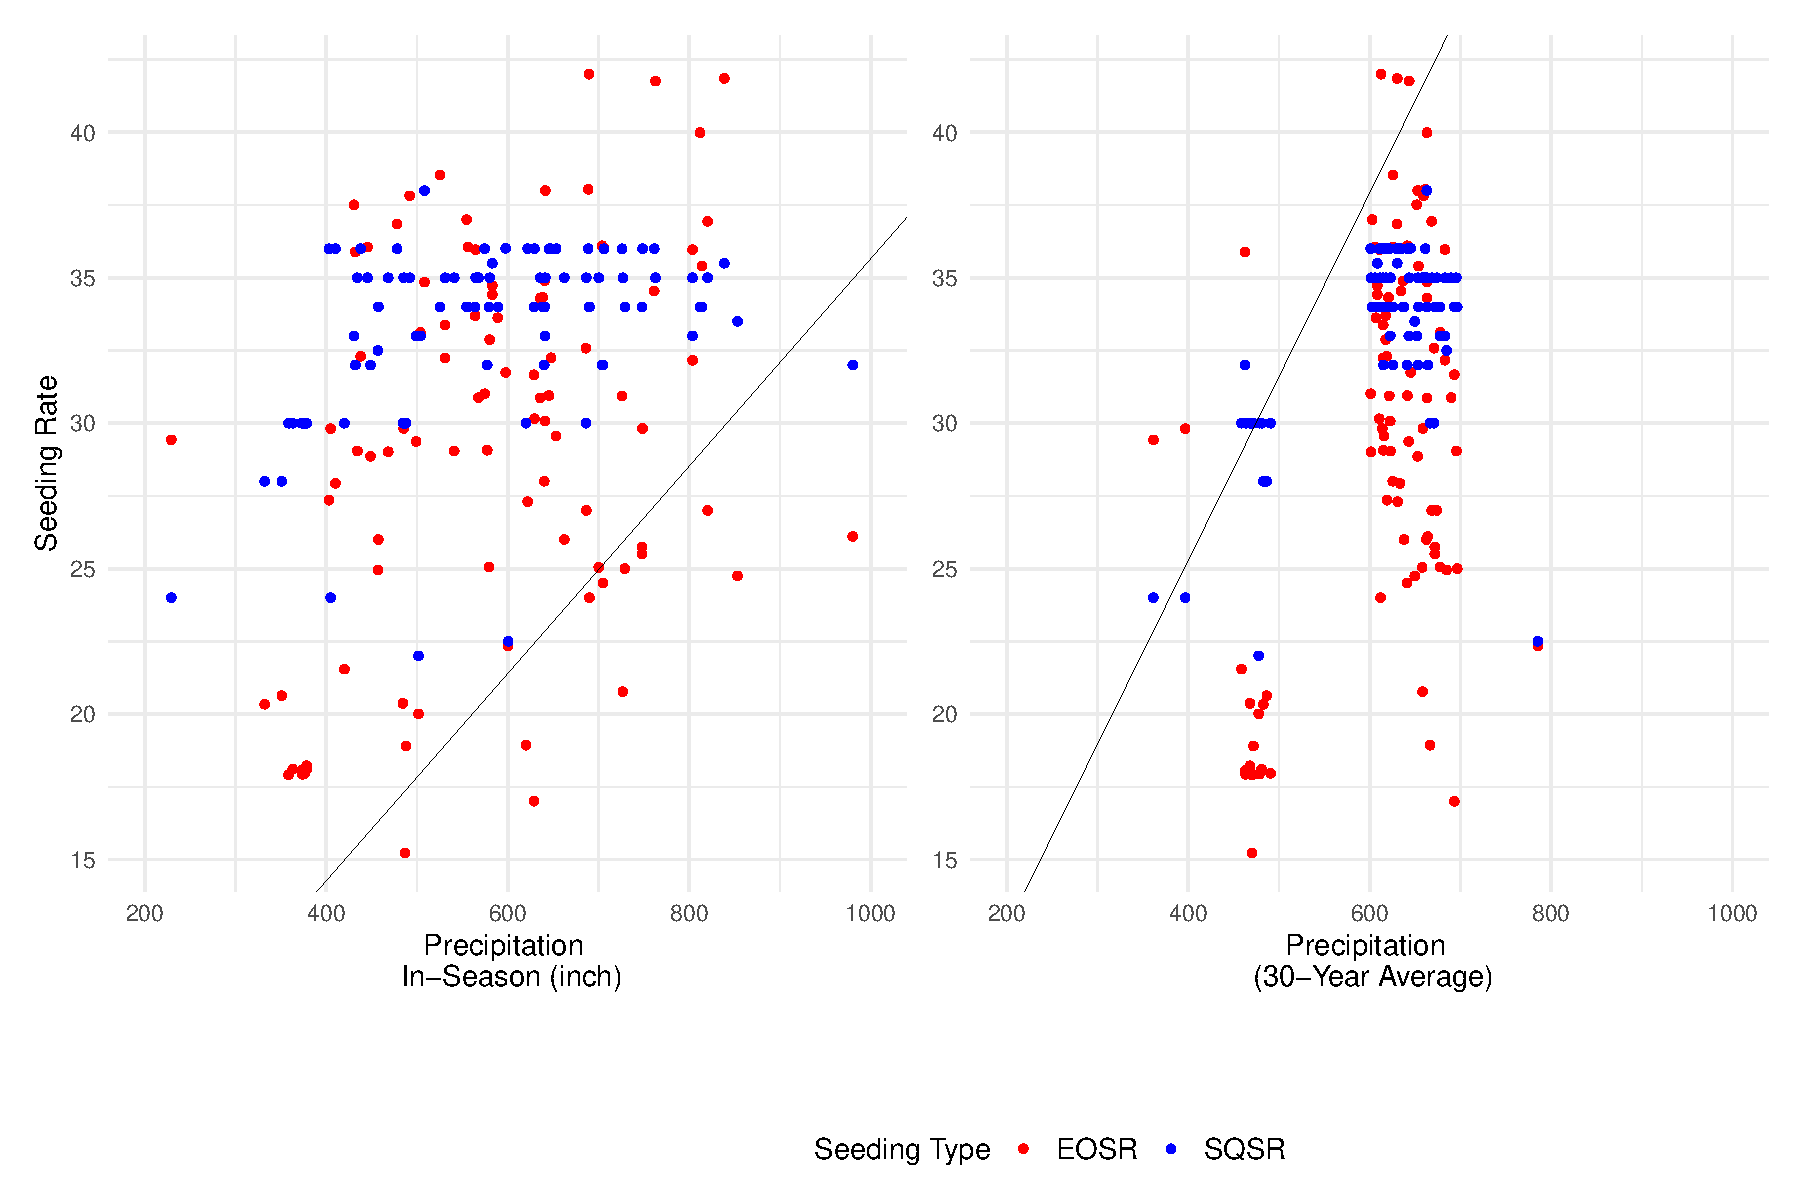
\includegraphics[width=17.1875in,height=\textheight]{corn_seed_response_writing_files/figure-pdf/fig3-eosr-sqsr-weather-1.pdf}

}

\caption{EOSR by In-season \& 30 year Avg Precipitation}

\end{figure}%

Figure
(\citeproc{ref-fig3-eosr-sqsr-weather}{\textbf{fig3-eosr-sqsr-weather?}})
illustrates the relationship between climate conditions and seeding
rates. The left panel compares EOSRs (red) and SQSRs (blue) based on
in-season total precipitation (inches) across 100 field trials, while
the right panel shows the comparison based on accumulated Growing Degree
Days (GDD). EOSRs exhibit greater vertical dispersion under the same
levels of precipitation or GDD, whereas SQSRs show less variation
relative to EOSRs. In 93 out of the 100 trials, SQSRs range from 30K to
36K, with a median value of 34K. In contrast, the median EOSR is 30.2K.

Additionally, Figure
(\citeproc{ref-fig3-eosr-sqsr-weather}{\textbf{fig3-eosr-sqsr-weather?}})
reveals that, across the 100 trials, farmers' seeding rates tend to be
higher than the estimated optimal, and this difference is skewed to the
left when projected onto the diagonal line (black), indicating a
tendency for over-seeding relative to the EOSR.

\global\setlength{\Oldarrayrulewidth}{\arrayrulewidth}

\global\setlength{\Oldtabcolsep}{\tabcolsep}

\setlength{\tabcolsep}{2pt}

\renewcommand*{\arraystretch}{1.5}



\providecommand{\ascline}[3]{\noalign{\global\arrayrulewidth #1}\arrayrulecolor[HTML]{#2}\cline{#3}}

\begin{longtable*}[c]{ccccccccc}



\ascline{1.5pt}{666666}{1-9}

\multicolumn{1}{>{}c}{\textcolor[HTML]{000000}{\fontsize{11}{11}\selectfont{resp\_type}}} & \multicolumn{1}{>{}c}{\textcolor[HTML]{000000}{\fontsize{11}{11}\selectfont{Field}}\textcolor[HTML]{000000}{\fontsize{11}{11}\selectfont{\linebreak }}\textcolor[HTML]{000000}{\fontsize{11}{11}\selectfont{Count}}} & \multicolumn{1}{>{}c}{\textcolor[HTML]{000000}{\fontsize{11}{11}\selectfont{Differences\ in\ }}\textcolor[HTML]{000000}{\fontsize{11}{11}\selectfont{\linebreak }}\textcolor[HTML]{000000}{\fontsize{11}{11}\selectfont{\ Seeding\ Rate}}\textcolor[HTML]{000000}{\fontsize{11}{11}\selectfont{\linebreak }}\textcolor[HTML]{000000}{\fontsize{11}{11}\selectfont{(K/ac)}}} & \multicolumn{1}{>{}c}{\textcolor[HTML]{000000}{\fontsize{11}{11}\selectfont{Differences\ in\ }}\textcolor[HTML]{000000}{\fontsize{11}{11}\selectfont{\linebreak }}\textcolor[HTML]{000000}{\fontsize{11}{11}\selectfont{\ Estimated\ Yield\ }}\textcolor[HTML]{000000}{\fontsize{11}{11}\selectfont{\linebreak }}\textcolor[HTML]{000000}{\fontsize{11}{11}\selectfont{\ (bu/ac)}}} & \multicolumn{1}{>{}c}{\textcolor[HTML]{000000}{\fontsize{11}{11}\selectfont{Differences\ in\ }}\textcolor[HTML]{000000}{\fontsize{11}{11}\selectfont{\linebreak }}\textcolor[HTML]{000000}{\fontsize{11}{11}\selectfont{\ Estimated\ Profit\ }}\textcolor[HTML]{000000}{\fontsize{11}{11}\selectfont{\linebreak }}\textcolor[HTML]{000000}{\fontsize{11}{11}\selectfont{\ (\$/ac)}}} & \multicolumn{1}{>{}c}{\textcolor[HTML]{000000}{\fontsize{11}{11}\selectfont{Precipitation}}\textcolor[HTML]{000000}{\fontsize{11}{11}\selectfont{\linebreak }}\textcolor[HTML]{000000}{\fontsize{11}{11}\selectfont{(In-Season)}}} & \multicolumn{1}{>{}c}{\textcolor[HTML]{000000}{\fontsize{11}{11}\selectfont{GDD}}\textcolor[HTML]{000000}{\fontsize{11}{11}\selectfont{\linebreak }}\textcolor[HTML]{000000}{\fontsize{11}{11}\selectfont{(In-Season)}}} & \multicolumn{1}{>{}c}{\textcolor[HTML]{000000}{\fontsize{11}{11}\selectfont{Precipitation}}\textcolor[HTML]{000000}{\fontsize{11}{11}\selectfont{\linebreak }}\textcolor[HTML]{000000}{\fontsize{11}{11}\selectfont{(30\ Year)}}} & \multicolumn{1}{>{}c}{\textcolor[HTML]{000000}{\fontsize{11}{11}\selectfont{GDD}}\textcolor[HTML]{000000}{\fontsize{11}{11}\selectfont{\linebreak }}\textcolor[HTML]{000000}{\fontsize{11}{11}\selectfont{(30\ Year)}}} \\

\ascline{1.5pt}{666666}{1-9}\endfirsthead 

\ascline{1.5pt}{666666}{1-9}

\multicolumn{1}{>{}c}{\textcolor[HTML]{000000}{\fontsize{11}{11}\selectfont{resp\_type}}} & \multicolumn{1}{>{}c}{\textcolor[HTML]{000000}{\fontsize{11}{11}\selectfont{Field}}\textcolor[HTML]{000000}{\fontsize{11}{11}\selectfont{\linebreak }}\textcolor[HTML]{000000}{\fontsize{11}{11}\selectfont{Count}}} & \multicolumn{1}{>{}c}{\textcolor[HTML]{000000}{\fontsize{11}{11}\selectfont{Differences\ in\ }}\textcolor[HTML]{000000}{\fontsize{11}{11}\selectfont{\linebreak }}\textcolor[HTML]{000000}{\fontsize{11}{11}\selectfont{\ Seeding\ Rate}}\textcolor[HTML]{000000}{\fontsize{11}{11}\selectfont{\linebreak }}\textcolor[HTML]{000000}{\fontsize{11}{11}\selectfont{(K/ac)}}} & \multicolumn{1}{>{}c}{\textcolor[HTML]{000000}{\fontsize{11}{11}\selectfont{Differences\ in\ }}\textcolor[HTML]{000000}{\fontsize{11}{11}\selectfont{\linebreak }}\textcolor[HTML]{000000}{\fontsize{11}{11}\selectfont{\ Estimated\ Yield\ }}\textcolor[HTML]{000000}{\fontsize{11}{11}\selectfont{\linebreak }}\textcolor[HTML]{000000}{\fontsize{11}{11}\selectfont{\ (bu/ac)}}} & \multicolumn{1}{>{}c}{\textcolor[HTML]{000000}{\fontsize{11}{11}\selectfont{Differences\ in\ }}\textcolor[HTML]{000000}{\fontsize{11}{11}\selectfont{\linebreak }}\textcolor[HTML]{000000}{\fontsize{11}{11}\selectfont{\ Estimated\ Profit\ }}\textcolor[HTML]{000000}{\fontsize{11}{11}\selectfont{\linebreak }}\textcolor[HTML]{000000}{\fontsize{11}{11}\selectfont{\ (\$/ac)}}} & \multicolumn{1}{>{}c}{\textcolor[HTML]{000000}{\fontsize{11}{11}\selectfont{Precipitation}}\textcolor[HTML]{000000}{\fontsize{11}{11}\selectfont{\linebreak }}\textcolor[HTML]{000000}{\fontsize{11}{11}\selectfont{(In-Season)}}} & \multicolumn{1}{>{}c}{\textcolor[HTML]{000000}{\fontsize{11}{11}\selectfont{GDD}}\textcolor[HTML]{000000}{\fontsize{11}{11}\selectfont{\linebreak }}\textcolor[HTML]{000000}{\fontsize{11}{11}\selectfont{(In-Season)}}} & \multicolumn{1}{>{}c}{\textcolor[HTML]{000000}{\fontsize{11}{11}\selectfont{Precipitation}}\textcolor[HTML]{000000}{\fontsize{11}{11}\selectfont{\linebreak }}\textcolor[HTML]{000000}{\fontsize{11}{11}\selectfont{(30\ Year)}}} & \multicolumn{1}{>{}c}{\textcolor[HTML]{000000}{\fontsize{11}{11}\selectfont{GDD}}\textcolor[HTML]{000000}{\fontsize{11}{11}\selectfont{\linebreak }}\textcolor[HTML]{000000}{\fontsize{11}{11}\selectfont{(30\ Year)}}} \\

\ascline{1.5pt}{666666}{1-9}\endhead



\multicolumn{1}{>{}c}{\textcolor[HTML]{000000}{\fontsize{11}{11}\selectfont{A1}}} & \multicolumn{1}{>{}c}{\textcolor[HTML]{000000}{\fontsize{11}{11}\selectfont{12}}} & \multicolumn{1}{>{}c}{\textcolor[HTML]{000000}{\fontsize{11}{11}\selectfont{-4.4}}\textcolor[HTML]{000000}{\fontsize{11}{11}\selectfont{\linebreak }}\textcolor[HTML]{000000}{\fontsize{11}{11}\selectfont{(2.2)}}} & \multicolumn{1}{>{}c}{\textcolor[HTML]{000000}{\fontsize{11}{11}\selectfont{-5.1}}\textcolor[HTML]{000000}{\fontsize{11}{11}\selectfont{\linebreak }}\textcolor[HTML]{000000}{\fontsize{11}{11}\selectfont{(2.8)}}} & \multicolumn{1}{>{}c}{\textcolor[HTML]{000000}{\fontsize{11}{11}\selectfont{-13.4}}\textcolor[HTML]{000000}{\fontsize{11}{11}\selectfont{\linebreak }}\textcolor[HTML]{000000}{\fontsize{11}{11}\selectfont{(12.3)}}} & \multicolumn{1}{>{}c}{\textcolor[HTML]{000000}{\fontsize{11}{11}\selectfont{611.6}}\textcolor[HTML]{000000}{\fontsize{11}{11}\selectfont{\linebreak }}\textcolor[HTML]{000000}{\fontsize{11}{11}\selectfont{(140.0)}}} & \multicolumn{1}{>{}c}{\textcolor[HTML]{000000}{\fontsize{11}{11}\selectfont{1781.7}}\textcolor[HTML]{000000}{\fontsize{11}{11}\selectfont{\linebreak }}\textcolor[HTML]{000000}{\fontsize{11}{11}\selectfont{(224.0)}}} & \multicolumn{1}{>{}c}{\textcolor[HTML]{000000}{\fontsize{11}{11}\selectfont{596.1}}\textcolor[HTML]{000000}{\fontsize{11}{11}\selectfont{\linebreak }}\textcolor[HTML]{000000}{\fontsize{11}{11}\selectfont{(80.9)}}} & \multicolumn{1}{>{}c}{\textcolor[HTML]{000000}{\fontsize{11}{11}\selectfont{1687.9}}\textcolor[HTML]{000000}{\fontsize{11}{11}\selectfont{\linebreak }}\textcolor[HTML]{000000}{\fontsize{11}{11}\selectfont{(206.7)}}} \\





\multicolumn{1}{>{}c}{\textcolor[HTML]{000000}{\fontsize{11}{11}\selectfont{A2}}} & \multicolumn{1}{>{}c}{\textcolor[HTML]{000000}{\fontsize{11}{11}\selectfont{12}}} & \multicolumn{1}{>{}c}{\textcolor[HTML]{000000}{\fontsize{11}{11}\selectfont{-2.2}}\textcolor[HTML]{000000}{\fontsize{11}{11}\selectfont{\linebreak }}\textcolor[HTML]{000000}{\fontsize{11}{11}\selectfont{(1.7)}}} & \multicolumn{1}{>{}c}{\textcolor[HTML]{000000}{\fontsize{11}{11}\selectfont{-2.4}}\textcolor[HTML]{000000}{\fontsize{11}{11}\selectfont{\linebreak }}\textcolor[HTML]{000000}{\fontsize{11}{11}\selectfont{(2.2)}}} & \multicolumn{1}{>{}c}{\textcolor[HTML]{000000}{\fontsize{11}{11}\selectfont{-5.3}}\textcolor[HTML]{000000}{\fontsize{11}{11}\selectfont{\linebreak }}\textcolor[HTML]{000000}{\fontsize{11}{11}\selectfont{(6.7)}}} & \multicolumn{1}{>{}c}{\textcolor[HTML]{000000}{\fontsize{11}{11}\selectfont{562.6}}\textcolor[HTML]{000000}{\fontsize{11}{11}\selectfont{\linebreak }}\textcolor[HTML]{000000}{\fontsize{11}{11}\selectfont{(160.7)}}} & \multicolumn{1}{>{}c}{\textcolor[HTML]{000000}{\fontsize{11}{11}\selectfont{1779.5}}\textcolor[HTML]{000000}{\fontsize{11}{11}\selectfont{\linebreak }}\textcolor[HTML]{000000}{\fontsize{11}{11}\selectfont{(216.7)}}} & \multicolumn{1}{>{}c}{\textcolor[HTML]{000000}{\fontsize{11}{11}\selectfont{622.6}}\textcolor[HTML]{000000}{\fontsize{11}{11}\selectfont{\linebreak }}\textcolor[HTML]{000000}{\fontsize{11}{11}\selectfont{(84.8)}}} & \multicolumn{1}{>{}c}{\textcolor[HTML]{000000}{\fontsize{11}{11}\selectfont{1714.8}}\textcolor[HTML]{000000}{\fontsize{11}{11}\selectfont{\linebreak }}\textcolor[HTML]{000000}{\fontsize{11}{11}\selectfont{(242.8)}}} \\





\multicolumn{1}{>{}c}{\textcolor[HTML]{000000}{\fontsize{11}{11}\selectfont{B1}}} & \multicolumn{1}{>{}c}{\textcolor[HTML]{000000}{\fontsize{11}{11}\selectfont{12}}} & \multicolumn{1}{>{}c}{\textcolor[HTML]{000000}{\fontsize{11}{11}\selectfont{9.4}}\textcolor[HTML]{000000}{\fontsize{11}{11}\selectfont{\linebreak }}\textcolor[HTML]{000000}{\fontsize{11}{11}\selectfont{(3.4)}}} & \multicolumn{1}{>{}c}{\textcolor[HTML]{000000}{\fontsize{11}{11}\selectfont{-8.2}}\textcolor[HTML]{000000}{\fontsize{11}{11}\selectfont{\linebreak }}\textcolor[HTML]{000000}{\fontsize{11}{11}\selectfont{(10.8)}}} & \multicolumn{1}{>{}c}{\textcolor[HTML]{000000}{\fontsize{11}{11}\selectfont{-74.5}}\textcolor[HTML]{000000}{\fontsize{11}{11}\selectfont{\linebreak }}\textcolor[HTML]{000000}{\fontsize{11}{11}\selectfont{(61.5)}}} & \multicolumn{1}{>{}c}{\textcolor[HTML]{000000}{\fontsize{11}{11}\selectfont{511.7}}\textcolor[HTML]{000000}{\fontsize{11}{11}\selectfont{\linebreak }}\textcolor[HTML]{000000}{\fontsize{11}{11}\selectfont{(190.3)}}} & \multicolumn{1}{>{}c}{\textcolor[HTML]{000000}{\fontsize{11}{11}\selectfont{1678.5}}\textcolor[HTML]{000000}{\fontsize{11}{11}\selectfont{\linebreak }}\textcolor[HTML]{000000}{\fontsize{11}{11}\selectfont{(167.7)}}} & \multicolumn{1}{>{}c}{\textcolor[HTML]{000000}{\fontsize{11}{11}\selectfont{557.8}}\textcolor[HTML]{000000}{\fontsize{11}{11}\selectfont{\linebreak }}\textcolor[HTML]{000000}{\fontsize{11}{11}\selectfont{(93.7)}}} & \multicolumn{1}{>{}c}{\textcolor[HTML]{000000}{\fontsize{11}{11}\selectfont{1563.7}}\textcolor[HTML]{000000}{\fontsize{11}{11}\selectfont{\linebreak }}\textcolor[HTML]{000000}{\fontsize{11}{11}\selectfont{(175.7)}}} \\





\multicolumn{1}{>{}c}{\textcolor[HTML]{000000}{\fontsize{11}{11}\selectfont{B2}}} & \multicolumn{1}{>{}c}{\textcolor[HTML]{000000}{\fontsize{11}{11}\selectfont{42}}} & \multicolumn{1}{>{}c}{\textcolor[HTML]{000000}{\fontsize{11}{11}\selectfont{5.3}}\textcolor[HTML]{000000}{\fontsize{11}{11}\selectfont{\linebreak }}\textcolor[HTML]{000000}{\fontsize{11}{11}\selectfont{(4.0)}}} & \multicolumn{1}{>{}c}{\textcolor[HTML]{000000}{\fontsize{11}{11}\selectfont{-1.7}}\textcolor[HTML]{000000}{\fontsize{11}{11}\selectfont{\linebreak }}\textcolor[HTML]{000000}{\fontsize{11}{11}\selectfont{(6.5)}}} & \multicolumn{1}{>{}c}{\textcolor[HTML]{000000}{\fontsize{11}{11}\selectfont{-26.3}}\textcolor[HTML]{000000}{\fontsize{11}{11}\selectfont{\linebreak }}\textcolor[HTML]{000000}{\fontsize{11}{11}\selectfont{(41.9)}}} & \multicolumn{1}{>{}c}{\textcolor[HTML]{000000}{\fontsize{11}{11}\selectfont{570.5}}\textcolor[HTML]{000000}{\fontsize{11}{11}\selectfont{\linebreak }}\textcolor[HTML]{000000}{\fontsize{11}{11}\selectfont{(115.4)}}} & \multicolumn{1}{>{}c}{\textcolor[HTML]{000000}{\fontsize{11}{11}\selectfont{1747.5}}\textcolor[HTML]{000000}{\fontsize{11}{11}\selectfont{\linebreak }}\textcolor[HTML]{000000}{\fontsize{11}{11}\selectfont{(172.8)}}} & \multicolumn{1}{>{}c}{\textcolor[HTML]{000000}{\fontsize{11}{11}\selectfont{620.8}}\textcolor[HTML]{000000}{\fontsize{11}{11}\selectfont{\linebreak }}\textcolor[HTML]{000000}{\fontsize{11}{11}\selectfont{(70.8)}}} & \multicolumn{1}{>{}c}{\textcolor[HTML]{000000}{\fontsize{11}{11}\selectfont{1677.0}}\textcolor[HTML]{000000}{\fontsize{11}{11}\selectfont{\linebreak }}\textcolor[HTML]{000000}{\fontsize{11}{11}\selectfont{(185.5)}}} \\





\multicolumn{1}{>{}c}{\textcolor[HTML]{000000}{\fontsize{11}{11}\selectfont{C}}} & \multicolumn{1}{>{}c}{\textcolor[HTML]{000000}{\fontsize{11}{11}\selectfont{18}}} & \multicolumn{1}{>{}c}{\textcolor[HTML]{000000}{\fontsize{11}{11}\selectfont{6.4}}\textcolor[HTML]{000000}{\fontsize{11}{11}\selectfont{\linebreak }}\textcolor[HTML]{000000}{\fontsize{11}{11}\selectfont{(4.5)}}} & \multicolumn{1}{>{}c}{\textcolor[HTML]{000000}{\fontsize{11}{11}\selectfont{-6.4}}\textcolor[HTML]{000000}{\fontsize{11}{11}\selectfont{\linebreak }}\textcolor[HTML]{000000}{\fontsize{11}{11}\selectfont{(9.7)}}} & \multicolumn{1}{>{}c}{\textcolor[HTML]{000000}{\fontsize{11}{11}\selectfont{-50.6}}\textcolor[HTML]{000000}{\fontsize{11}{11}\selectfont{\linebreak }}\textcolor[HTML]{000000}{\fontsize{11}{11}\selectfont{(60.5)}}} & \multicolumn{1}{>{}c}{\textcolor[HTML]{000000}{\fontsize{11}{11}\selectfont{643.3}}\textcolor[HTML]{000000}{\fontsize{11}{11}\selectfont{\linebreak }}\textcolor[HTML]{000000}{\fontsize{11}{11}\selectfont{(149.5)}}} & \multicolumn{1}{>{}c}{\textcolor[HTML]{000000}{\fontsize{11}{11}\selectfont{1799.5}}\textcolor[HTML]{000000}{\fontsize{11}{11}\selectfont{\linebreak }}\textcolor[HTML]{000000}{\fontsize{11}{11}\selectfont{(208.6)}}} & \multicolumn{1}{>{}c}{\textcolor[HTML]{000000}{\fontsize{11}{11}\selectfont{621.9}}\textcolor[HTML]{000000}{\fontsize{11}{11}\selectfont{\linebreak }}\textcolor[HTML]{000000}{\fontsize{11}{11}\selectfont{(69.1)}}} & \multicolumn{1}{>{}c}{\textcolor[HTML]{000000}{\fontsize{11}{11}\selectfont{1709.0}}\textcolor[HTML]{000000}{\fontsize{11}{11}\selectfont{\linebreak }}\textcolor[HTML]{000000}{\fontsize{11}{11}\selectfont{(189.6)}}} \\

\ascline{1.5pt}{666666}{1-9}



\end{longtable*}



\arrayrulecolor[HTML]{000000}

\global\setlength{\arrayrulewidth}{\Oldarrayrulewidth}

\global\setlength{\tabcolsep}{\Oldtabcolsep}

\renewcommand*{\arraystretch}{1}

For a more detailed evaluation of farmers' seeding rate decisions, table
(\citeproc{ref-tab2-result-resp-type}{\textbf{tab2-result-resp-type?}})
presents the differences in seeding rate, yield, and profit at the SQSR
and EOSR, with the 100 trials divided into five categories. These
categories are based on the concavity of the yield response function,
the sign of the difference between SQSR and EOSR, and whether the EOSR
matches the Yield Maximizing Seeding Rate (YMSR).

The concavity of the yield response function is a crucial factor in
economic analysis, as a convex response typically results in a corner
solution at either the minimum or maximum value of the input, providing
little useful guidance for determining an optimal seeding rate. In
contrast, when the EOSR equals the YMSR, in some cases, the EOSR may
also occur at the minimum or maximum of the trial input range. In these
instances, the EOSR offers limited insight, as it only applies within
the specific range of inputs used in the trial.

In table
(\citeproc{ref-tab2-result-resp-type}{\textbf{tab2-result-resp-type?}})
,the overall difference between the SQSRs and EOSRs averages -3.8K,
meaning that, on average, farmers are seeding 3.8K more seeds per acre
than the estimated optimal rate. The estimated yield at SQSRs is 3.4
bushels per acre less than at EOSRs, reflecting the diminishing yield
effect when seeding rates exceed the EOSR. Types A1 and B1 represent
trials where the yield response function is concave, but the EOSR is
identical to the YMSR. In many A1 type trials, the EOSRs are at or near
the maximum of the trial input range, while in B1 type trials, the EOSRs
are at or near the minimum of the trial input range. The average seeding
rate differences are -4.5K in A1 and 9.1K in B1, indicating that, in the
24 trials classified as A1 and B1, farmers tend to choose higher seeding
rates than the EOSR. The average yield difference between A1 and B1 is
3.1 bushels per acre, but the estimated profit difference between these
groups is \$69.3 per acre. This result highlights that the potential
profit loss from farmers' SQSR choices is largely due to the cost of
excessive seeding. However, because some trials have EOSRs at the
extremes of the input range (either the maximum or minimum), the numeric
results for groups A1 and B1 may be biased.

Types A2 and B2 represent trials where the EOSRs are the most accurate
and informative, as the yield response functions are concave, and the
EOSRs are neither at the maximum nor the minimum of the trial input
ranges. In these groups, the average yield difference between the two is
only 1.5 bushels per acre, but the estimated profit difference is \$18.8
per acre. Notably, the B2 group comprises 41 out of the 100 total
trials, indicating that farmers tend to plant excessive seeds in many
cases. This over-seeding leads to significant profit losses due to
unproductive investment in seed.

\begin{figure}[H]

{\centering 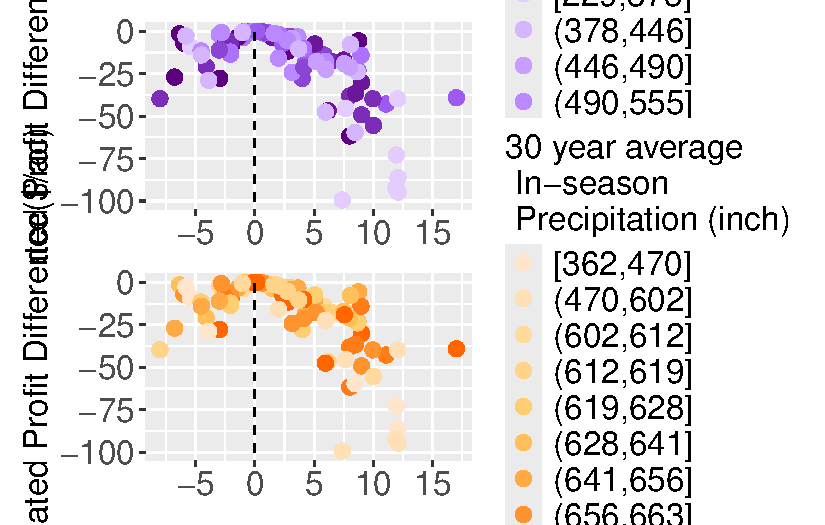
\includegraphics[width=17.1875in,height=\textheight]{corn_seed_response_writing_files/figure-pdf/fig4-dif-pro-seed-comb-1.pdf}

}

\caption{Difference in estimated Profit at a given climate condition by
seeding status (SQSR-EOSR)}

\end{figure}%

Figure
(\citeproc{ref-fig4-dif-pro-seed-comb}{\textbf{fig4-dif-pro-seed-comb?}})
displays the differences in Estimated Profit and Seeding Rate between
the SQSR and EOSR , with the top panel showing these differences as a
function of total in-sesaon precipitation of the trial year and the
bottom panel categorizing them by the 30 year average precipitation of
the trial region. This figure provides a visual representation of the
results in
(\citeproc{ref-tab2-result-resp-type}{\textbf{tab2-result-resp-type?}})
, illustrating the individual observations (trials) across both
dimensions.

Figure (\citeproc{ref-fig5-rest-type-all}{\textbf{fig5-rest-type-all?}})
visualizes the reasons why the estimated profits of the B2 group are
significantly lower than those of the A2 group. The figures in the first
row illustrate how the YMSR can lead to profit losses when compared to
thecEOSR. In the right figure of the first row, the estimated profit
response curve is flatter than the yield response curve, highlighting
how a flatter profit curve contributes to potential profit losses at the
YMSR. In the Type B2 group, the yield response to seeding follows a
quadratic pattern, plateauing beyond the YMSR. However, the profit
response to seeding diminishes rapidly beyond the YMSR, which explains
the potential loss of profit due to excessive seeding. Additionally, in
several B2 trials, the yield response is not a quadratic plateau but a
quadratic diminishing curve. As a result, profits decrease more sharply
with higher seeding rates in these fields. In the Type A1 and B1 groups,
as shown in the figures in the bottom row, many trials have their EOSRs
at either the minimum or maximum of the trial input range.

\section{Discussion}\label{discussion}

The tables and figures in the results section present the estimated
yield and profit based on a fixed crop and seed price ratio of \$5.5 per
bushel of corn and \$3.8 per thousand seeds. To further evaluate
farmers' seeding decisions across different response types under varying
crop and seed price ratios, estimated yield and profit were also
calculated based on the annual price ratio changes over the past 10
years.

Figure
(\citeproc{ref-fig6-dif-pro-seed-by-price}{\textbf{fig6-dif-pro-seed-by-price?}})
shows the estimated profit for each response type under the highest
relative seed cost (top) and the lowest relative seed cost (bottom).
When comparing these figures with Figure
(\citeproc{ref-fig4-dif-pro-seed-by-comb}{\textbf{fig4-dif-pro-seed-by-comb?}})
, more trials fall into the A1 and A2 categories under the lowest
relative seed cost. However, even with lower relative seed costs, the
estimated profit loss due to excessive seeding rates (to the right of
the black dashed vertical line) remains higher than the loss from
deficient seeding rates.

\section{Conclusion}\label{conclusion}

This study evaluates the estimated profit of farmers' SQSR and EOSR in
corn production across the U.S. Midwest corn belt, focusing on potential
profit losses from over- or under-seeding behavior of farmers. The
analysis, based on 100 on-farm trials conducted from 2016 to 2023,
reveals that many farmers tend to over-seed, choosing seeding rates
(SQSR) higher than the estimated EOSR. The median SQSR is 34K seeds per
acre, compared to an EOSR of 30.2K, resulting in a yield difference of
3.4 bu/ac and an average profit loss of \$18.8 to \$69.3 per acre
depending on the response type.

Farmers' higher-than-optimal seeding rates, driven by past
recommendations or their own experience, are often not adjusted to
current economic and environmental conditions. Despite variations in
yield responses, excessive seeding consistently leads to diminishing
returns due to rising seed costs, which have approached fertilizer costs
in recent decades. The findings highlight that reducing seeding rates in
fields with high estimated profit losses can significantly enhance
profitability, especially as seed prices continue to rise. By better
understanding the yield response to seeding rates and adjusting
practices accordingly, farmers can minimize unnecessary input costs and
maximize profit, particularly under increasingly frequent droughts and
high-temperature events.

\section*{References}\label{references}
\addcontentsline{toc}{section}{References}

\phantomsection\label{refs}
\begin{CSLReferences}{0}{1}
\bibitem[\citeproctext]{ref-usdanass}
\CSLLeftMargin{1. }%
\CSLRightInline{U. NASS, Census of agriculture, crop production
historical track records. \emph{www.nass.usda.gov/AgCensus} (2024).}

\bibitem[\citeproctext]{ref-morris2018strengths}
\CSLLeftMargin{2. }%
\CSLRightInline{T. F. Morris, \emph{et al.}, Strengths and limitations
of nitrogen rate recommendations for corn and opportunities for
improvement. \emph{Agronomy journal} \textbf{110}, 1--37 (2018).}

\bibitem[\citeproctext]{ref-fernandez2014genetically}
\CSLLeftMargin{3. }%
\CSLRightInline{J. Fernandez-Cornejo, S. Wechsler, M. Livingston, L.
Mitchell, Genetically engineered crops in the united states.
\emph{USDA-ERS Economic Research Report} (2014).}

\bibitem[\citeproctext]{ref-saavoss2021trends}
\CSLLeftMargin{4. }%
\CSLRightInline{M. Saavoss, T. Capehart, W. McBride, A. Effland, Trends
in production practices and costs of the US corn sector.
\emph{10.22004/ag.econ.312954} (2021).}

\bibitem[\citeproctext]{ref-illinois2023seed}
\CSLLeftMargin{5. }%
\CSLRightInline{E. D. Nafziger, G. P. Fontes, Planting corn in 2023.
\emph{Department of Crop Sciences, University of Illinois} (2023).}

\bibitem[\citeproctext]{ref-licht2017corn}
\CSLLeftMargin{6. }%
\CSLRightInline{M. A. Licht, A. W. Lenssen, R. W. Elmore, Corn (zea mays
l.) seeding rate optimization in iowa, USA. \emph{Precision Agriculture}
\textbf{18}, 452--469 (2017).}

\bibitem[\citeproctext]{ref-lindsey2018modeling}
\CSLLeftMargin{7. }%
\CSLRightInline{A. J. Lindsey, P. R. Thomison, E. D. Nafziger, Modeling
the effect of varied and fixed seeding rates at a small-plot scale.
\emph{Agronomy Journal} \textbf{110}, 2456--2461 (2018).}

\bibitem[\citeproctext]{ref-nielsen2019yield}
\CSLLeftMargin{8. }%
\CSLRightInline{R. Nielsen, J. Lee, J. Hettinga, J. Camberato, Yield
response of corn to plant population in indiana. \emph{Purdue University
Department of Agronomy Applied Crop Production Research Update} (2019).}

\bibitem[\citeproctext]{ref-lacasa2020bayesian}
\CSLLeftMargin{9. }%
\CSLRightInline{J. Lacasa, \emph{et al.}, Bayesian approach for maize
yield response to plant density from both agronomic and economic
viewpoints in north america. \emph{Scientific reports} \textbf{10},
15948 (2020).}

\bibitem[\citeproctext]{ref-assefa2018analysis}
\CSLLeftMargin{10. }%
\CSLRightInline{Y. Assefa, \emph{et al.}, Analysis of long term study
indicates both agronomic optimal plant density and increase maize yield
per plant contributed to yield gain. \emph{Scientific Reports}
\textbf{8}, 4937 (2018).}

\bibitem[\citeproctext]{ref-kukal2018climate}
\CSLLeftMargin{11. }%
\CSLRightInline{M. S. Kukal, S. Irmak, Climate-driven crop yield and
yield variability and climate change impacts on the US great plains
agricultural production. \emph{Scientific reports} \textbf{8}, 1--18
(2018).}

\bibitem[\citeproctext]{ref-rigden2020combined}
\CSLLeftMargin{12. }%
\CSLRightInline{A. Rigden, N. Mueller, N. Holbrook, N. Pillai, P.
Huybers, Combined influence of soil moisture and atmospheric evaporative
demand is important for accurately predicting US maize yields.
\emph{Nature Food} \textbf{1}, 127--133 (2020).}

\bibitem[\citeproctext]{ref-bullock2019data}
\CSLLeftMargin{13. }%
\CSLRightInline{D. S. Bullock, \emph{et al.}, The data-intensive farm
management project: Changing agronomic research through on-farm
precision experimentation. \emph{Agronomy Journal} \textbf{111},
2736--2746 (2019).}

\bibitem[\citeproctext]{ref-lix2021design}
\CSLLeftMargin{14. }%
\CSLRightInline{X. Li, Taro Mieno, D. S. Bullock, The economic
performances of different trial designs in on-farm precision
experimentation: A monte carlo evaluation. \emph{Working paper} (2021).}

\bibitem[\citeproctext]{ref-edge2024processing}
\CSLLeftMargin{15. }%
\CSLRightInline{B. Edge, T. Mieno, D. S. Bullock, Processing of on-farm
precision experiment data in the DIFM project. \emph{Center for Open
Science} (2024).}

\bibitem[\citeproctext]{ref-r2021language}
\CSLLeftMargin{16. }%
\CSLRightInline{R. C. Team, \emph{et al.}, A language and environment
for statistical computing. \emph{https://www.R-project.org/} (2021).}

\bibitem[\citeproctext]{ref-thornton2022daymet}
\CSLLeftMargin{17. }%
\CSLRightInline{M. Thornton, \emph{et al.}, Daymet: Monthly climate
summaries on a 1-km grid for north america, version 4 R1. ORNL DAAC, oak
ridge, tennessee, USA. \emph{https://doi.org/10.3334/ORNLDAAC/2131}
(2022).}

\end{CSLReferences}




\end{document}
